\documentclass{tufte-handout}
\usepackage[utf8]{inputenc}
\usepackage[francais]{babel}

\title{Manuel d'utilisation du simulateur ARM epater\\Révision 2}


\author{Marc-André Gardner, Yannick Hold-Geoffroy et Jean-François Lalonde}

%\date{28 March 2010} % without \date command, current date is supplied

%\geometry{showframe} % display margins for debugging page layout

\usepackage{graphicx} % allow embedded images
  \setkeys{Gin}{width=\linewidth,totalheight=\textheight,keepaspectratio}
  \graphicspath{{graphics/}} % set of paths to search for images
\usepackage{amsmath}  % extended mathematics
\usepackage{booktabs} % book-quality tables
\usepackage{units}    % non-stacked fractions and better unit spacing
\usepackage{multicol} % multiple column layout facilities
\usepackage{lipsum}   % filler text
\usepackage{fancyvrb} % extended verbatim environments
  \fvset{fontsize=\normalsize}% default font size for fancy-verbatim environments

% Standardize command font styles and environments
\newcommand{\doccmd}[1]{\texttt{\textbackslash#1}}% command name -- adds backslash automatically
\newcommand{\docopt}[1]{\ensuremath{\langle}\textrm{\textit{#1}}\ensuremath{\rangle}}% optional command argument
\newcommand{\docarg}[1]{\textrm{\textit{#1}}}% (required) command argument
\newcommand{\docenv}[1]{\textsf{#1}}% environment name
\newcommand{\docpkg}[1]{\texttt{#1}}% package name
\newcommand{\doccls}[1]{\texttt{#1}}% document class name
\newcommand{\docclsopt}[1]{\texttt{#1}}% document class option name
\newenvironment{docspec}{\begin{quote}\noindent}{\end{quote}}% command specification environment
\usepackage{hyperref}


\usepackage{color}


\begin{document}

\maketitle% this prints the handout title, author, and date

\section{Introduction}

Ce manuel présente l'utilisation du simulateur \textbf{épater}, qui émule un processeur à architecture ARMv4 (coeur ARM7), tel qu'étudié dans le cours \textit{GIF-1001 Ordinateurs: Structure et Applications}. Il présente également succinctement le jeu d'instruction ARMv4. Des informations complémentaires concernant l'architecture ARM et la programmation en assembleur peuvent être obtenues dans les notes de cours ou dans les manuels de référence cités dans le plan de cours.

\section{Prise en main}

\subsection{Accès au simulateur}

Le simulateur est disponible à l'adresse \url{http://gif1001-sim.gel.ulaval.ca/}. Aucune installation n'est nécessaire. Le simulateur a été testé avec les navigateurs suivants :
\begin{itemize}
	\item Google Chrome version 50 et plus, sur Windows, MacOS et Linux
	\item Mozilla Firefox version 44 et plus, sur Windows, MacOS et Linux
	\item Microsoft Edge, sur Windows 10
	\item Apple Safari, sur MacOS
\end{itemize}

D'autres navigateurs peuvent également être compatibles avec l'interface du simulateur, mais cette compatibilité n'est pas garantie. Si vous rencontrez des problèmes avec un navigateur alternatif, installez un des navigateurs énumérés plus haut.


\paragraph{\textbf{\color{red}{Note importante :}}} {\color{red}{Le simulateur opère automatiquement une sauvegarde \textbf{locale} de votre code. Aucune donnée n'est conservée sur le serveur : si les données de votre navigateur sont effacées ou perdues, vous \textbf{perdrez} votre code. Veillez à \textbf{toujours} télécharger le fichier contenant votre code, en utilisant le bouton ``Sauvegarder'', à chaque fois que vous quittez la session de simulation ou fermez votre navigateur. Il est de \textbf{votre} responsabilité de vous assurer de conserver ces fichiers en lieu sûr. L'équipe du simulateur ne pourra être tenue responsable de perte de données et \textbf{ne possède aucun moyen} de récupérer des données perdues.}}

%Le serveur sauvegarde automatiquement votre code, mais il n'y a aucune garantie que celui-ci sera conservé après avoir quitté la session de simulation. Il est de \emph{votre} responsabilité de télécharger le fichier contenant votre code à chaque fois que vous quittez la session de simulation ou fermez votre navigateur.}}


\tableofcontents

\clearpage
\section{Utilisation du simulateur}

La page d'accueil du simulateur est présentée à la figure \ref{f:accueil}. Elle contient, sur la gauche, un menu permettant de choisir le type d'activité (démonstrations, exercices, travaux pratiques ou simulation libre) et, dans sa section principale, une liste des programmes disponibles.

\begin{figure}
\raggedleft
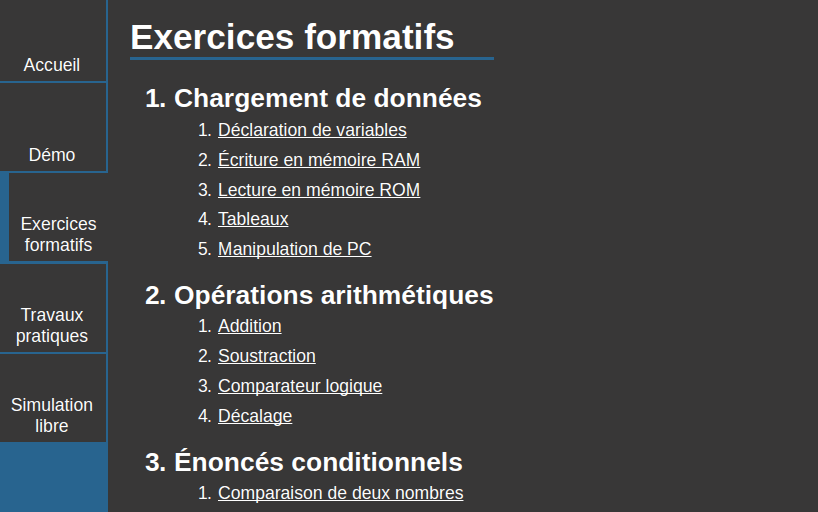
\includegraphics[width=0.7\linewidth]{pics/accueil.png}
\label{f:accueil}
\caption{Page d'accueil du simulateur}
\end{figure}

Cliquer sur l'un de ces programmes ouvre l'interface de simulation à proprement parler. La figure \ref{f:global} présente un exemple typique de cette interface, annotée. Les sous-sections suivantes présentent chaque zone de l'interface.

\begin{figure*}[h!]
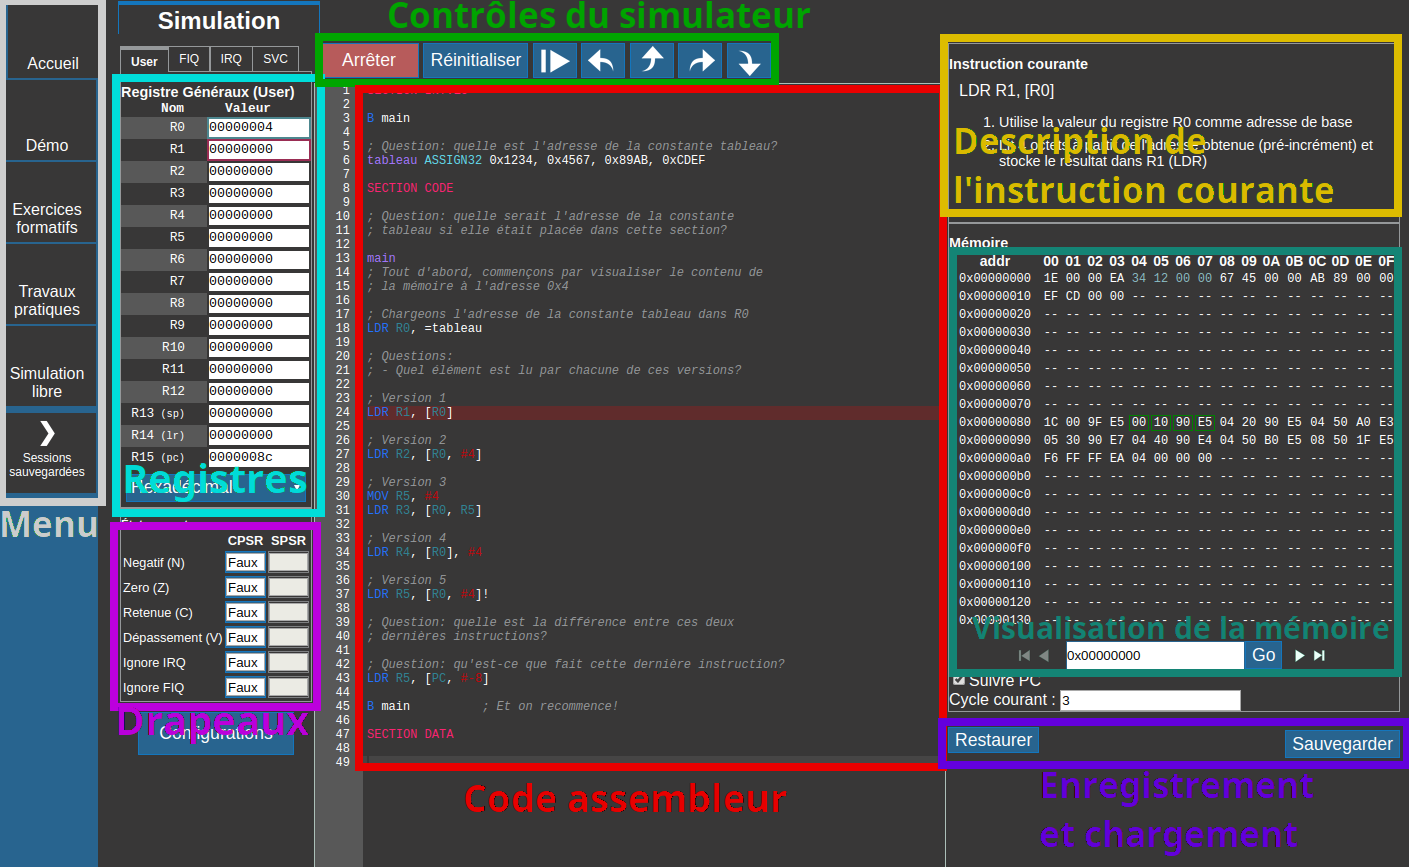
\includegraphics[width=0.86\linewidth]{pics/main_labeled.png}
\label{f:global}
\caption{Vue d'ensemble de l'interface du simulateur.}
\end{figure*}

\clearpage

\subsection{Éditeur de code}

\begin{marginfigure}
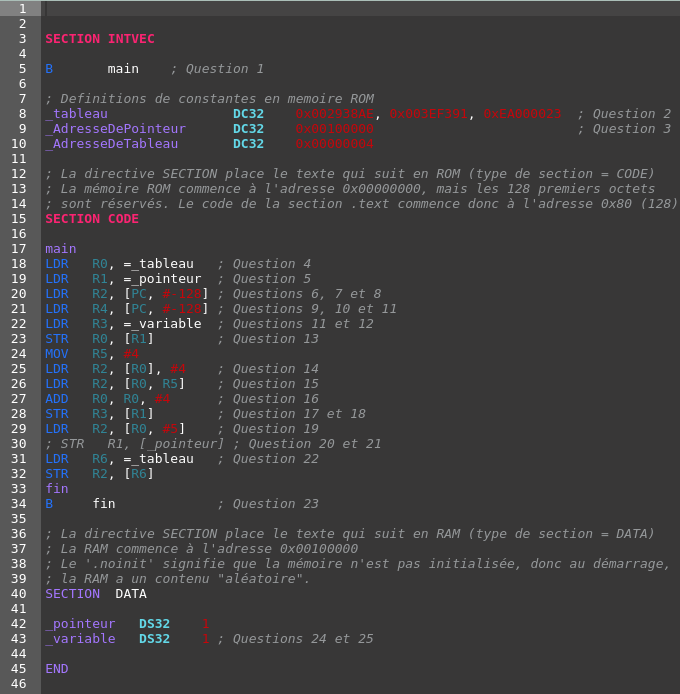
\includegraphics[width=\linewidth]{pics/editeur.png}
\label{f:editeur}
\caption{Vue typique de l'éditeur}
\end{marginfigure}
L'éditeur de code constitue la zone principale du simulateur. C'est dans cet éditeur que vous pouvez créer votre programme. Lors de l'exécution, \emph{l'éditeur passe en mode lecture seulement}, mais présente certaines informations comme la ligne en cours d'exécution.

Cet éditeur possède une \emph{coloration syntaxique}, c'est-à-dire qu'il est capable d'analyser le code qu'il convient pour colorier différemment les diverses parties d'une instructions. Cela permet de faciliter la lecture et la détection des erreurs. 

La colonne de gauche contient le numéro de ligne. Lorsqu'une instruction est erronée, un X blanc sur fond rouge y apparaît pour signaler le problème :
\begin{figure}[h!]
\raggedleft
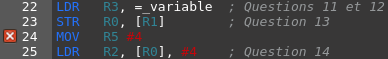
\includegraphics[width=0.9\linewidth]{pics/editeur_err.png}
\label{f:editeurerror}
\caption{Exemple d'instruction erronée. Le X blanc sur fond rouge signale la ligne contenant l'instruction invalide.}
\end{figure}

Passer la souris sur ce X fait apparaître une infobulle contenant un texte explicatif de l'erreur :
\begin{figure}[h!]
\raggedleft
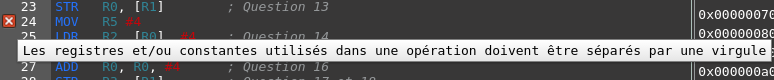
\includegraphics[width=\linewidth]{pics/editeur_err_bulle.png}
\label{f:editeurerrorplus}
\caption{Le message expliquant l'erreur peut être consulté en passant la souris sur le X.}
\end{figure}


Il est possible de mettre en place des points d'arrêt (\textit{breakpoints}) en cliquant sur le numéro d'une ligne. Un point d'arrêt force le simulateur à s'arrêter lorsqu'il l'atteint. Un point d'arrêt peut être désactivé en recliquant sur le même numéro de ligne. Par exemple, dans la figure suivante, les lignes 20 et 22 sont des points d'arrêt :
\begin{figure}[h!]
\raggedleft
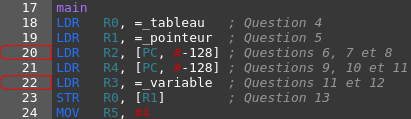
\includegraphics[width=0.9\linewidth]{pics/editeur_bkpt.png}
\label{f:editeurbkpt}
\caption{Un point d'arrêt (\textit{breakpoint}) peut être mis en place en cliquant sur le numéro de ligne.}
\end{figure}

\paragraph{\textbf{Note importante :}}un point d'arrêt peut être placé sur n'importe quelle ligne si le programme n'est \emph{pas assemblé}. Une fois le programme \emph{assemblé} (le bouton ``Démarrer'' pressé et le code assemblé sans erreur), un point d'arrêt peut seulement être placé sur une ligne \emph{contenant une instruction} et un point d'arrêt invalide est désactivé ou déplacé sur la prochaine ligne. Si l'utilisateur clique sur une ligne ne contenant pas d'instruction, le point d'arrêt sera placé sur la prochaine ligne contenant une instruction. Par exemple, à la figure \ref{f:editeurbkpt}, cliquer sur la ligne 17 placera un point d'arrêt à la ligne \emph{18}.

Lors de l'exécution, l'éditeur passe en mode lecture seule. Il affiche cependant certaines informations. La ligne en cours d'exécution est surlignée en rouge bourgogne :
\begin{figure}[h!]
\raggedleft
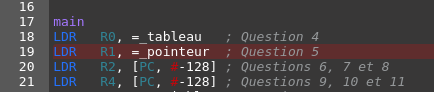
\includegraphics[width=0.9\linewidth]{pics/editeur_lignecourante.png}
\label{f:editeurlignecourante}
\caption{L'instruction qui va être exécutée au prochain pas de temps est surlignée en rouge dans l'éditeur. Si aucune instruction n'est surlignée, c'est que le \textit{Program Counter} (PC) ne se situe pas dans la mémoire d'instructions.}
\end{figure}

De même, lorsque l'instruction courante est un branchement ou un appel de fonction, l'éditeur affiche la destination du branchement en surlignant en noir la prochaine instruction. Par exemple, dans ce cas-ci, l'instruction en cours d'exécution (surlignée en rouge) est le \textit{B main}, et la prochaine instruction sera celle de la ligne 18 (surlignée en noir) :
\begin{figure}[h!]
\raggedleft
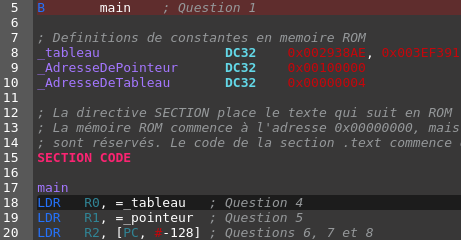
\includegraphics[width=0.9\linewidth]{pics/editeur_prediction.png}
\label{f:editeurbranch}
\caption{La prochaine instruction à être exécutée après un branchement est surlignée en noir profond. Si le branchement est conditionnel, cet affichage en tient compte et affiche la prochaine instruction correspondant à la branche prise.}
\end{figure}

\clearpage

\subsection{Contrôles du simulateur}

Les boutons de contrôle du simulateur permettent d'agir sur la simulation. 
Cette interface diffère selon le mode actuel. Dans le mode \emph{édition} (figure~\ref{f:controles1}), seul le bouton \textit{Démarrer} est actif. Dans le mode \emph{exécution}, que l'on peut accéder en pressant sur \textit{Démarrer}, tous les boutons sont actifs, et le bouton \textit{Démarrer} devient \textit{Arrêter}. 
\begin{figure}[h!]
\raggedleft

\includegraphics[width=0.8\linewidth]{pics/controles_1b.png}
\label{f:controles1}
\caption{Barre de contrôle en mode \emph{édition}}
\end{figure}
\vspace{-1em}
\begin{figure}[h!]
\raggedleft

\includegraphics[width=0.8\linewidth]{pics/controles_2b.png}
\label{f:controles2}
\caption{Barre de contrôle en mode \emph{exécution}}
\end{figure}

Lorsque le bouton \textit{Démarrer} est pressé, le simulateur tente d'abord d'assembler le code. Si aucune erreur n'est détectée, il passe alors en mode exécution. Dans ce mode, tous les boutons sont actifs et sont, respectivement, de gauche à droite :
\begin{enumerate}
	\item \textbf{Arrêt} : interrompt la simulation et revient en mode édition.
	\item \textbf{Réinitialisation} : effectue l'équivalent d'une interruption \emph{reset} sur le microprocesseur. La valeur de PC est mise à $0$. Notez que cela n'affecte \emph{pas} la valeur des autres registres et des drapeaux.
	\item \textbf{Exécution en continu} : le simulateur exécute les instructions suivantes sans arrêt, jusqu'à ce qu'il rencontre une erreur ou un point d'arrêt. Notez que le simulateur est volontairement limité quant au nombre d'instructions qu'il peut exécuter d'un seul coup (10\,000). Lorsque ce nombre est atteint, le simulateur arrête comme s'il avait rencontré un point d'arrêt. Il suffit d'appuyer à nouveau sur le bouton d'exécution en continu pour poursuivre.
    \item \textbf{Retour en arrière} : retourne en arrière d'une instruction. L'état du simulateur (les registres, la mémoire et les drapeaux) retourne comme il était à l'instruction précédente puis arrête.
	\item \textbf{Exécuter jusqu'à la sortie} : dans le cas où la ligne courante est dans une fonction, cette action exécute sans arrêt les instructions jusqu'à sortir de la fonction (appel de BX). Si la ligne courante n'est pas dans une fonction, cette action a le même effet qu'une exécution en continu.
	\item \textbf{Exécuter ligne courante} : dans le cas où la ligne courante est une instruction autre que BL, cette action a le même effet que la précédente. Toutefois, dans le cas d'un appel de fonction (BL), cette action exécute l'entièreté de la fonction jusqu'à son retour.
	\item \textbf{Exécuter instruction courante} : exécute l'instruction courante (celle qui est surlignée dans l'éditeur) et passe à la suivante puis arrête.
\end{enumerate}

\clearpage

\subsection{Vue des registres}

\begin{marginfigure}
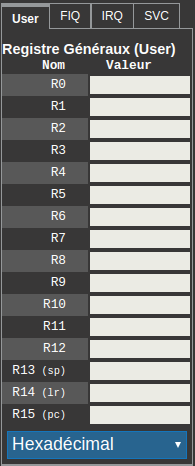
\includegraphics[width=0.8\linewidth]{pics/registres.png}
\label{f:registres}
\caption{Vue des registres généraux}
\end{marginfigure}
La section de gauche de l'interface présente les valeurs contenues dans les registres du processeur.
Les 16 registres que contient un processeur ARM (R0 à R15) sont affichés. 

Par défaut, leur valeur est présentée en hexadécimal, mais il est possible de choisir différents modes d'affichage en cliquant sur le mode actuel pour faire apparaître le menu de sélection. Le mode décimal signé correspond à une interprétation complément-2 de la valeur du registre, alors que le mode non-signé correspond à une simple conversion vers le système décimal.
\begin{marginfigure}
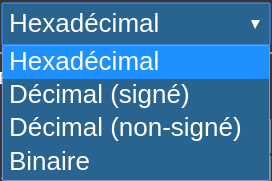
\includegraphics[width=0.8\linewidth]{pics/registres_format.png}
\label{f:regformat}
\caption{Menu de sélection du mode d'affichage}
\end{marginfigure}

Les onglets au-dessus des registres permettent de choisir la \textit{banque} de registre à visualiser. La plupart des banques de registre d'un processeur ARM sont présentes, incluant la banque IRQ (interruption), FIQ (interruption rapide) et SVC (interruption logicielle).
\begin{marginfigure}

\includegraphics[width=\linewidth]{pics/registres_banques.png}
\label{f:regbank}
\caption{Onglets de sélection de la banque de registres à visualiser}
\end{marginfigure}

La valeur d'un registre peut être modifiée en changeant sa valeur dans l'interface. Attention toutefois à respecter le type d'affichage sélectionné (par exemple, il est illégal d'écrire autre chose que 0 ou 1 en mode binaire).

Il est possible d'affecter un point d'arrêt à un registre, en mode lecture ou écriture. Un point d'arrêt lié à un registre met la simulation en pause lorsque le registre est écrit ou lu. Par exemple, dans la figure suivante, les registres R3 et R5 ont un point d'arrêt en écriture et le registre R2 un point d'arrêt en lecture :
\begin{marginfigure}
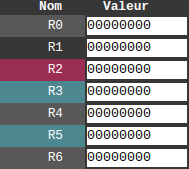
\includegraphics[width=0.8\linewidth]{pics/registres_bkpt.png}
\label{f:regbkpt}
\caption{Points d'arrêt sur les registres R2, R3 et R5.}
\end{marginfigure}

Un point d'arrêt en écriture peut être ajouté en cliquant sur le nom du registre tout en tenant la touche Ctrl ou Cmd enfoncée, respectivement sur Windows et MacOS. De même, un point d'arrêt en lecture peut être ajouté en cliquant tout en tenant la touche Maj (Shift) enfoncée. Un point d'arrêt précédemment créé peut être retiré en répétant la même opération. Il est possible de mettre à la fois un point d'arrêt en lecture et en écriture sur le même registre.

Lorsque l'instruction courante lit ou écrit un registre, sa valeur est entourée d'un rectangle turquoise (lecture) ou rouge (écriture). Par exemple, dans l'image suivante, l'instruction courante lit les valeurs de R0 et R5 et écrit dans R2 :
\begin{figure}[h!]
\raggedright
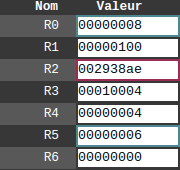
\includegraphics[width=0.38\linewidth]{pics/registres_statuts.png}
\label{f:regstatut}
\end{figure}

\clearpage

\subsection{Vue des drapeaux}

Les drapeaux de l'ALU sont présentés juste en dessous de la vue des registres.
\begin{marginfigure}
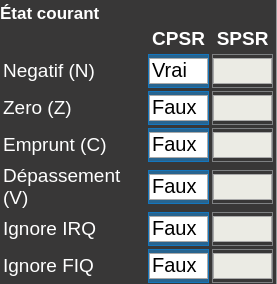
\includegraphics[width=0.9\linewidth]{pics/drapeaux.png}
\label{f:drapeaux}
\caption{Vue des drapeaux de l'ALU}
\end{marginfigure} 
Un drapeau ne peut prendre que deux valeurs : vrai ou faux (0 ou 1 en binaire). Il est possible de changer la valeur d'un drapeau en cliquant sur sa valeur. L'interface présente à la fois la vue pour le registre de statut courant (CPSR) et le registre de statut sauvegardé (SPSR), si applicable.

Le registre de statut sauvegardé (SPSR) est propre à chaque banque de registres, hormis la banque \textit{User} qui n'en possède pas. Il permet de conserver le registre de statut du programme principal pendant une interruption. Dans la majorité des cas (exécution en mode \textit{User}), les valeurs du SPSR ne sont pas définies ou modifiables.

Tout comme pour les registres, les drapeaux lus ou écrits par une instructions voient leur contour coloré de manière différente.

\clearpage

\subsection{Vue de la mémoire}
 
La vue de la mémoire présente le contenu de la mémoire d'instructions et de données. Cette vue est arrangée en tableau, où chaque ligne fait 16 octets de largeur.
Par exemple, pour retrouver la valeur à l'adresse $0$x9A, il suffit d'aller au croisement de la ligne $0$x90 et de la colonne $0$xA.
Les espaces mémoire non déclarés (qui ne se rapportent ni à une instruction, ni à une variable) sont indiqués par des tirets. L'affichage du contenu de la mémoire se fait en hexadécimal.
\begin{marginfigure}
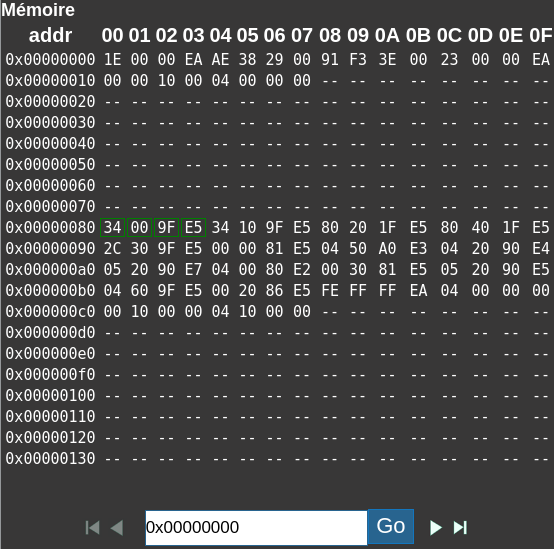
\includegraphics[width=0.9\linewidth]{pics/memoire.png}
\label{f:memoire}
\caption{Vue de la mémoire}
\end{marginfigure}
Tout comme pour les registres et les drapeaux, il est possible de modifier une valeur initialisée de la mémoire en cliquant. Les zones non déclarées (dont la valeur est identifiée par des tirets) ne peuvent être modifiées. La valeur doit être écrite en hexadécimal et ne peut excéder la capacité d'un octet (255, soit $0$xFF).

Lors de l'exécution, les octets composant l'instruction courante (celle surlignée en rouge dans l'éditeur) sont entourés de vert, comme dans l'exemple suivant :
\begin{figure}[h!]
\raggedleft
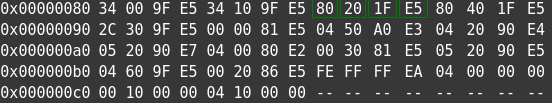
\includegraphics[width=0.8\linewidth]{pics/memoire_pc.png}
\label{f:memoirepc}
\caption{Affichage des octets composant l'instruction courante}
\end{figure}

Lorsque l'instruction est une opération agissant en mémoire, les cases mémoires lues ou écrites voient leurs valeurs colorées de manière différente (vert dans le cas d'une lecture, rouge dans le cas d'une écriture). Par exemple, dans l'image suivante, l'instruction courante lit les valeurs $0$x10 à $0$x13 inclusivement :
\begin{figure}[h!]
\raggedleft
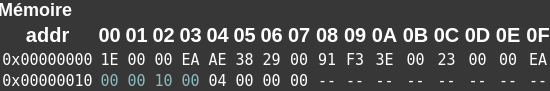
\includegraphics[width=0.8\linewidth]{pics/memoire_acces.png}
\label{f:memoireacces}
\caption{Exemple du changement de couleur des valeurs d'une case mémoire lors d'un accès}
\end{figure}

Il est possible de placer des points d'arrêt en mémoire. Ceux-ci peuvent être de trois types :
\begin{itemize}
	\item \textbf{Lecture} : le simulateur s'arrête lorsqu'un accès en lecture (par exemple via l'instruction LDR) est effectué sur cette case mémoire
	\item \textbf{Écriture} : le simulateur s'arrête lorsqu'un accès en écriture (par exemple via l'instruction STR) est effectué sur cette case mémoire
	\item \textbf{Exécution} : le simulateur s'arrête lorsque le \textit{Program Counter} (PC) atteint cette valeur
\end{itemize}
Notons que ces trois types de points d'arrêt peuvent être combinés. Par exemple, dans l'image suivante, un point d'arrêt en lecture est présent pour les adresses $0$x04 à $0$x07, un point d'arrêt en écriture est actif aux adresses $0$x0C à $0$x0F et un point d'arrêt en exécution est présent à l'adresse $0$x8C :
\begin{figure}[h!]
\raggedleft
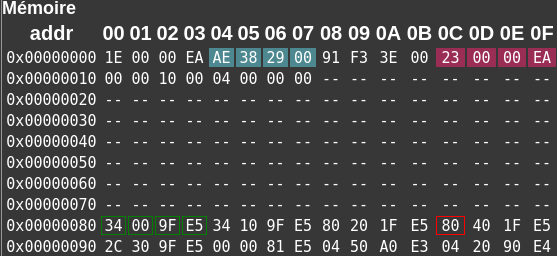
\includegraphics[width=0.8\linewidth]{pics/memoire_bkpt.png}
\label{f:memoirebkpt}
\caption{Exemple de points d'arrêt en mémoire. Un point d'arrêt en lecture peut être ajouté en cliquant sur une case mémoire tout en pressant la touche Control (Ctrl). Un point d'arrêt en écriture peut être ajouté en cliquant et pressant la touche Maj (Shift). Un point d'arrêt en écriture peut être ajouté en cliquant et pressant la touche Alt.}
\end{figure}

Afin de faciliter l'utilisation du simulateur, un aide-mémoire succinct reprenant les informations présentées ici est disponible en bas de la vue mémoire :
\begin{figure}[h!]
\raggedleft
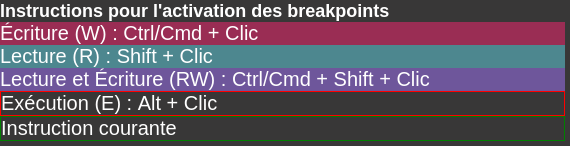
\includegraphics[width=0.6\linewidth]{pics/memoire_reminder.png}
\label{f:memoirerem}
\caption{Description des différents types de points d'arrêt en mémoire dans l'interface du simulateur}
\end{figure}

Finalement, en bas du visualisateur, on retrouve une interface permettant de naviguer dans la mémoire :
\begin{figure}[h!]
\raggedleft

\includegraphics[width=0.6\linewidth]{pics/memoire_goto.png}
\label{f:memoiregoto}
\caption{Contrôle de la position dans la mémoire}
\end{figure}

 Les flèches permettent d'aller vers des adresses mémoire plus hautes ou plus basses. Le champ de texte central permet de spécifier directement une adresse, à laquelle on peut par la suite se rendre en pressant le bouton \textit{Go}.
 
Finalement, notons que cette vue indique, par un soulignement blanc, la position en mémoire de la ligne couramment \textit{sélectionnée} dans l'éditeur (celle sur laquelle se trouve le curseur). Si cette ligne est une instruction, elle couvrira 4 cases (soit 4 octets). S'il s'agit plutôt d'une constante ou d'une variable, elle indiquera toutes les cases mémoire appartenant à de celle-ci. 
 \begin{figure}[h!]
\raggedleft
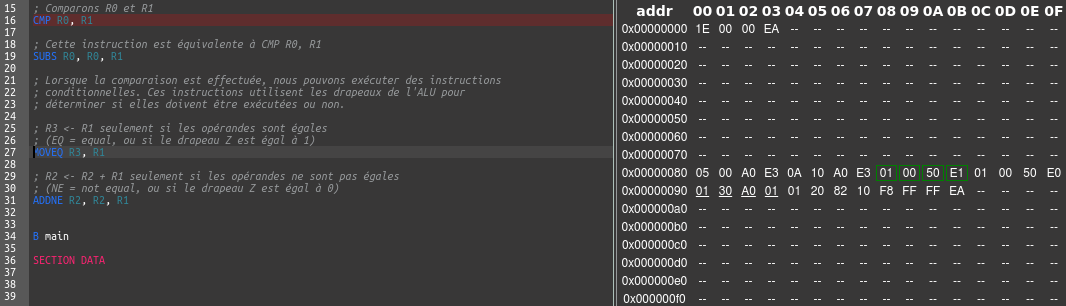
\includegraphics[width=0.98\linewidth]{pics/memoire_courant.png}
\label{f:memoirecurrent}
\caption{Vue de la position de la ligne couramment sélectionnée. Dans ce cas-ci, la ligne 27 est sélectionnée; la vue mémoire souligne en blanc les cases mémoires qui y correspondent, soit les adresses 0x90 à 0x93 inclusivement. La ligne en cours d'exécution est quant à elle surlignée en rouge et sa position en mémoire indiquée par des carrés verts autour des cases concernées.}
\end{figure}

\clearpage

\subsection{Description de l'instruction courante}

Cette section présente des informations textuelles sur l'instruction courante. La première ligne présente l'instruction \emph{désassemblée} : elle provient non pas de l'éditeur, mais du \textit{bytecode} lui-même. Cela lui permet d'apporter de l'information supplémentaire dans deux circonstances :
\begin{enumerate}
	\item Les étiquettes y sont remplacées par les décalages effectifs requis pour atteindre la case mémoire demandée
	\item Dans le cas où l'on exécute des données présentes en mémoire, auxquelles aucun code assembleur n'est lié, cet affichage reste fonctionnel puisqu'il ne se base que sur la représentation binaire des instructions.
\end{enumerate}
\begin{figure}[h!]
\raggedleft
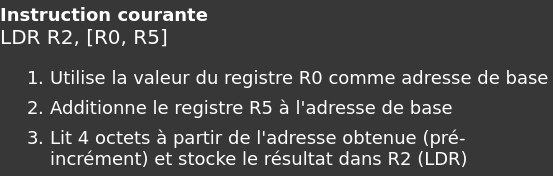
\includegraphics[width=0.6\linewidth]{pics/disassembly.png}
\label{f:disassembly}
\caption{Affichage de l'instruction désassemblée et de sa description. En fonction de l'instruction, la description peut être plus ou moins longue.}
\end{figure}

Les lignes suivantes sont une description textuelle de l'instruction, générée automatiquement. Elles indiquent, dans l'ordre, les opérations effectuées pour obtenir le résultat final et leurs effets de bord s'il y a lieu. Dans le cas d'une instruction indéfinie, cette zone reste vide.


\clearpage
\subsection{Sauvegarde des sessions de travail}

Les sessions sauvegardées permettent d'alterner entre plusieurs versions de code d'une même simulation. La session courante est sauvegardée automatiquement et restaurée au retour à la même simulation. 

\begin{figure}[h!]
\raggedleft
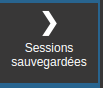
\includegraphics[width=0.2\linewidth]{pics/session_button.png}
\label{f:session_button}
\caption{Boutton du menu latéral}
\end{figure}

Pour afficher le panneau des sessions sauvegardées, il faut survoler le bouton ``Sessions sauvegardées'' du menu latéral. 

\begin{figure}[h!]
\raggedleft
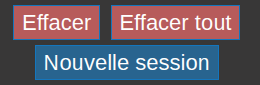
\includegraphics[width=0.4\linewidth]{pics/session_control.png}
\label{f:session_control}
\caption{Contrôle des sessions sauvegardées}
\end{figure}

Trois bouton sont accessible pour modifier les sessions : 
\begin{enumerate}     
\item \textbf{Effacer} : la session courante est supprimée et la suivante est sélectionnée (son code est restauré).
\item \textbf{Effacer tout} : toutes les sessions sont supprimées puis le code par défaut est restauré.
\item \textbf{Nouvelle session} : la session courante est sauvegardée et une nouvelle session est ajoutée en tête de la liste. Le code par défaut est restauré. 
\end{enumerate}

\begin{marginfigure}
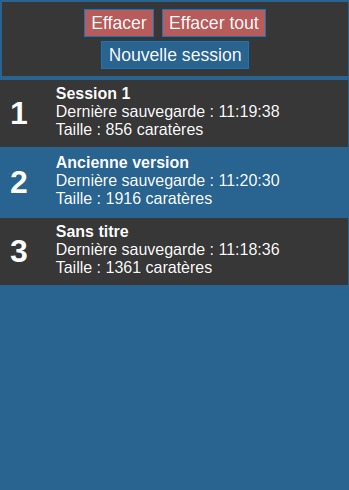
\includegraphics[width=\linewidth]{pics/session_open.png}
\label{f:session_open}
\caption{Vue des sessions sauvegardées avec la session numéro 2 de sélectionnée}
\end{marginfigure}

De plus, cliquer sur une session sauvegarde la session courante et restaure la session sélectionnée. La session en cours est affichée en bleu pour la différencier.

Certaines informations sont affichées pour distinguer les différentes sessions. On y retrouve le numéro de la session, l'heure de la dernière sauvegarde, la taille du code (en nombre de caractères) et le nom personnalisé de la session. Un double-clic sur le nom permet de le modifier.

\paragraph{\textbf{Note importante :}} bien que ce procédé permette de sauvegarder son code même après la fermeture de votre navigateur, \textbf{il est fortement recommandé d'enregistrer (télécharger) votre code}. Les sauvegardes de sessions sont enregistrées dans la mémoire de votre navigateur et il n'y a aucune garantie que celle-ci ne sera pas effacée. Si c'est le cas, l'équipe du simulateur ne possède aucun moyen de récupérer votre code, puisque aucune donnée n'est enregistrée sur le serveur.  

\clearpage
\subsection{Contrôles d'enregistrement et de chargement}

Ces contrôles, situés au bas de l'écran, vous permettent de télécharger le code présent dans l'éditeur et de charger un code présent sur votre ordinateur. Ces deux actions sont analogues à l'ouverture et l'enregistrement dans une application traditionnelle.

\begin{figure}[h!]
\raggedleft
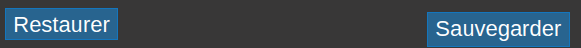
\includegraphics[width=0.9\linewidth]{pics/opensave.png}
\label{f:opensave}
\caption{Interface d'ouverture et d'enregistrement}
\end{figure}

N'importe quel type de fichier texte brut peut être lu par le simulateur. Nous vous recommandons toutefois d'utiliser l'extension ``txt'' afin d'éviter la confusion avec d'autres formats de fichier. C'est d'ailleurs cette extension que comportent les fichiers téléchargés depuis le simulateur.

\paragraph{\textbf{Note importante :}}malgré que votre code est sauvegarder automatiquement dans votre navigateur, \textbf{il est fortement recommandé de sauvegarder votre code} avec ces contrôles.

\clearpage
\subsection{Configuration}

La fenêtre de configuration peut être ouverte en pressant le bouton \textit{Configurations} situé sous la vue des drapeaux. Une fois ouverte, la fenêtre ressemble à celle-ci :
\begin{figure}[h!]
\raggedleft
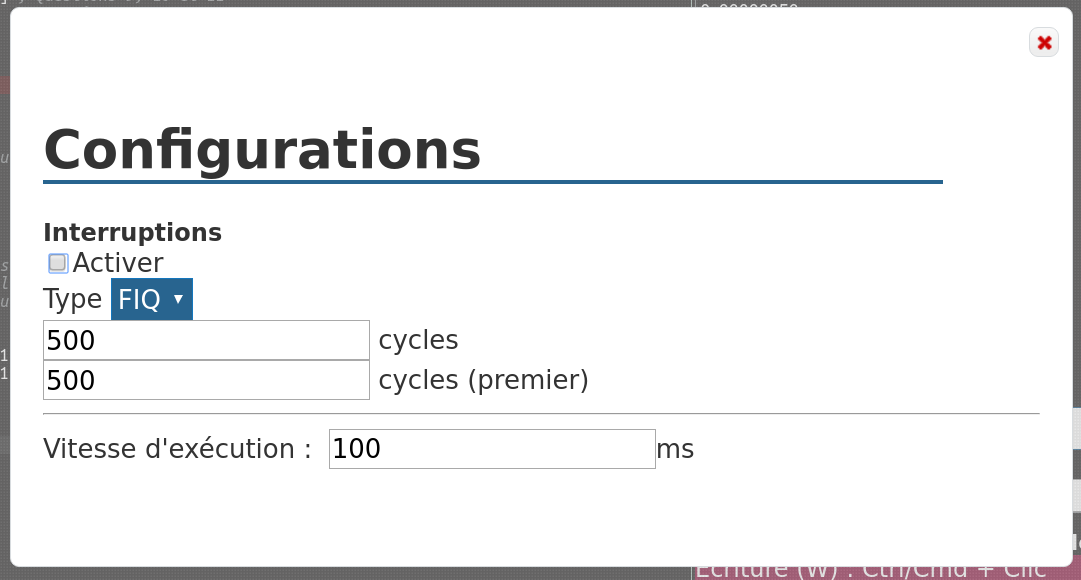
\includegraphics[width=0.9\linewidth]{pics/configurations.png}
\label{f:config}
\caption{Interface de configuration des interruptions et du simulateur}
\end{figure}

Deux éléments principaux peuvent être configurés dans cette interface :
\begin{enumerate}
	\item Une interruption temporelle peut être activée, en mode FIQ ou IRQ. Le nombre de cycles avant la première interruption, de même que le délai de répétition (encore là en nombre de cycles processeur) peuvent être configurés.
	\item La vitesse d'exécution, qui correspond au délai minimum entre l'exécution de deux instructions consécutives. Par défaut, cette vitesse est de 0, c'est-à-dire que le simulateur exécute les instructions aussi vite que possible. Toutefois, il est possible d'augmenter ce délai afin de pouvoir visualiser l'exécution du programme. Dans tous les cas, le simulateur se met automatiquement en pause après avoir exécuté 10\,000 instructions de suite.
\end{enumerate}

\clearpage
\section{Instructions ARM supportées}

Le simulateur supporte toutes les instructions ARMv4 à l'exception des instructions du co-processeur. Elles sont présentées dans les sections suivantes. Référez-vous aux notes de cours ou à la documentation d'ARM pour plus de détails sur chacune de celles-ci. La syntaxe à utiliser est celle présentée dans les spécifications et documentations techniques d'ARM, sauf pour les spécificités suivantes :
\begin{enumerate}
	\item Toutes les mnémoniques (MOV, LDR, BL, etc.) doivent être écrites en \textbf{majuscules}
	\item Tous les noms de registres doivent être écrits en \textbf{majuscules}
	\item Les étiquettes peuvent contenir, majuscules, minuscules et chiffres, mais pas \textit{commencer} par un chiffre.
	\item L'indentation n'a pas d'importance. L'espace ou la tabulation après la mnémonique est obligatoire.
%	\item Une \emph{section} se déclare uniquement par son nom. Les attributs de section (par exemple \textit{.noinit}) ne sont pas supportés.

\end{enumerate}


\noindent Toutes les instructions peuvent être exécutées \emph{conditionnellement}, en ajoutant un des codes à 2 lettres suivants à la fin de la mnémonique :
\vspace{-0.8em}
\begin{table}
\begin{tabular}{l|p{2cm}p{6cm}l}
Code & Équation & Explication & Signé? \\ \hline
\textbf{EQ}	& $A == B$ & Teste l'égalité & N/A \\
\textbf{NE}	& $A \neq B$ & Teste l'inégalité & N/A \\ \hline
\textbf{CS}	& $A \geq B$ & Teste si un premier nombre est plus grand ou égal à un second & NON \\
\textbf{CC}	& $A < B$ & Teste si un premier nombre est strictement plus petit qu'un second & NON \\
\textbf{HI}	& $A > B$ & Teste si un premier nombre est strictement plus grand qu'un second & NON \\
\textbf{LS}	& $A \leq B$ & Teste si un premier nombre est plus petit ou égal à un second & NON \\ \hline
\textbf{GE}	& $A \geq B$ & Teste si un premier nombre est plus grand ou égal à un second & OUI \\
\textbf{LT}	& $A < B$ & Teste si un premier nombre est strictement plus petit qu'un second & OUI \\
\textbf{GT}	& $A > B$ & Teste si un premier nombre est strictement plus grand qu'un second & OUI \\
\textbf{LE}	& $A \leq B$ & Teste si un premier nombre est plus petit ou égal à un second & OUI \\ \hline
\textbf{MI}	& $A < 0$ & Teste si le résultat est négatif & OUI \\
\textbf{PL}	& $A \geq 0$ & Teste si le résultat est positif & OUI \\ \hline
\textbf{VS}	& N/A & Teste si la précédente opération a généré un \textit{débordement} (overflow) & OUI \\
\textbf{VC}	& N/A & Teste si la précédente opération \textbf{n'a pas} généré un \textit{débordement} (overflow) & OUI \\ \hline
%\textbf{AL}	& N/A & Exécute systématiquement l'instruction (pas de condition, implicite) & N/A \\
\end{tabular}
\caption{Codes de condition en ARM. Notons qu'une condition spéciale (AL) est implicitement ajoutée à n'importe quelle instruction ne comportant pas de condition. Cette condition signifie que l'instruction doit être inconditionnellement exécutée. La colonne \textit{Signé?} indique si la comparaison présume un nombre signé ou non. Par exemple, la condition CS considère que les nombres ne sont pas signés, si bien que comparer -1 (0xFFFFFFFF) et 0 (0x00000000) sera vrai, comme si $-1 \geq 0$. À l'opposé, la condition GE tient compte du bit de signe et sera fausse pour cette même comparaison.}
\end{table}

\clearpage

\section{Instructions de données}

Les instructions manipulant les données peuvent accepter deux ou trois arguments. Lorsque le dernier argument est un registre, il peut optionnellement être décalé par une constante ou un autre registre avant d'exécuter le reste de l'instruction (voir le tableau \ref{t:decalage}). Le résultat de l'exécution de l'instruction peut également affecter les drapeaux, en ajoutant le suffixe \textit{S} à la mnémonique.

Les instructions de manipulation de données peuvent être divisées en quatre catégories :

\begin{itemize}
	\item Les instructions arithmétiques : voir tableau \ref{t:dataarith} 
	\item Les instructions booléennes et logiques : voir tableau \ref{t:databool}
	\item Les instructions arithmétiques utilisant la valeur du drapeau retenue C (\textit{Carry}) : voir tableau \ref{t:dataarithwithcarry}
	\item Les instructions de comparaison (arithmétiques et booléennes) : voir tableau \ref{t:datacmp}
\end{itemize}

\subsection{Exemples d'utilisation}

\paragraph{\texttt{MOV R1, R2}} Copie la valeur du registre R2 dans le registre R1.
\paragraph{\texttt{MOV R0, \#8}} Écrit la valeur 8 dans le registre R0.
\paragraph{\texttt{MOVEQ R3, R4}} Copie la valeur du registre R4 dans le registre R3 seulement si la condition EQ est vraie.
\paragraph{\texttt{MOV R3, R4, LSL \#4}} Copie la valeur du registre R4 décalée de 4 bits vers la gauche dans le registre R3.
\paragraph{\texttt{MOV R3, R4, LSR R5}} Copie la valeur du registre R4 décalée de $N$ bits vers la droite, où $N$ est la valeur de R5, dans le registre R3.

\paragraph{\texttt{ADD R8, PC, \#0x10}} Ajoute 16 (0x10) à PC, met le résultat dans R8.
\paragraph{\texttt{SUBS R0, R4, R5}} Soustrait R4 et R5, stocke le résultat dans R0 et met à jour les drapeaux en fonction de ce résultat.
\paragraph{\texttt{ADD R0, R1, R2, LSL \#1}} Additionne R1 et la valeur de R2 décalée de une position vers la gauche, stocke le résultat dans R0.
\paragraph{\texttt{RSBNES SP, R8, R9, ASR R7}} Soustrait la valeur de R9, décalée arithmétiquement vers la droite R7 fois, et R8, stocke le résultat dans SP et met à jour les drapeaux en fonction de ce résultat, mais seulement si la condition NE est rencontrée.



\begin{table*}
\begin{tabular}{l|l|p{13.5cm}}
Type & Format & Effet \\ \hline
\textbf{LSL} & \texttt{LSL N} & Décale les bits vers la \textbf{gauche} N fois. Des zéros sont insérés à droite pour remplacer les bits décalés. Le bit qui se retrouverait immédiatement à gauche du MSB devient la valeur du drapeau de retenue C (\textit{Carry}) si le suffixe \textit{S} est utilisé.

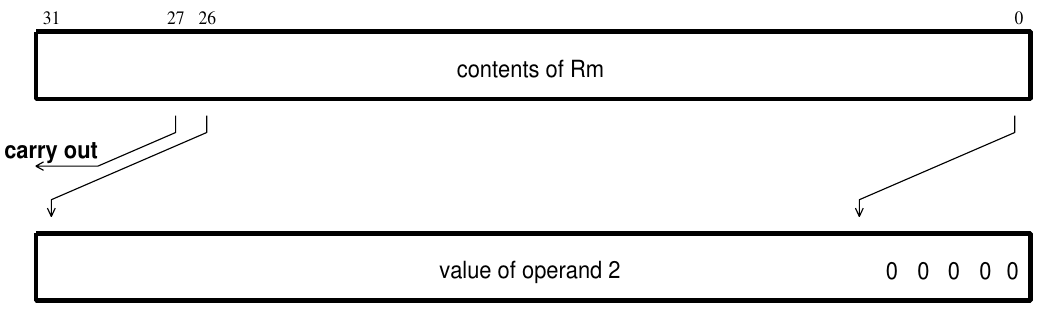
\includegraphics[width=9cm]{pics/lsl.png} \\  \hline

\textbf{LSR} & \texttt{LSR N} & Décale les bits vers la \textbf{droite} N fois. Des zéros sont insérés à gauche pour remplacer les bits décalés. Le bit qui se retrouverait immédiatement à droite du LSB devient la valeur du drapeau de retenue C (\textit{Carry}) si le suffixe \textit{S} est utilisé.

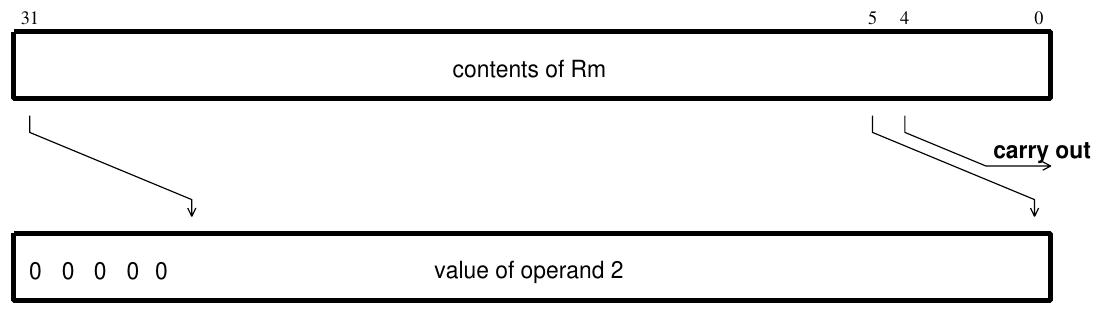
\includegraphics[width=9cm]{pics/lsr.png} \\  \hline

\textbf{ASR} & \texttt{ASR N} & Décale les bits vers la \textbf{droite} N fois. Les bits insérés à gauche ont la même valeur que le MSB actuel (bit 31). Le bit qui se retrouverait immédiatement à droite du LSB devient la valeur du drapeau de retenue C (\textit{Carry}) si le suffixe \textit{S} est utilisé.

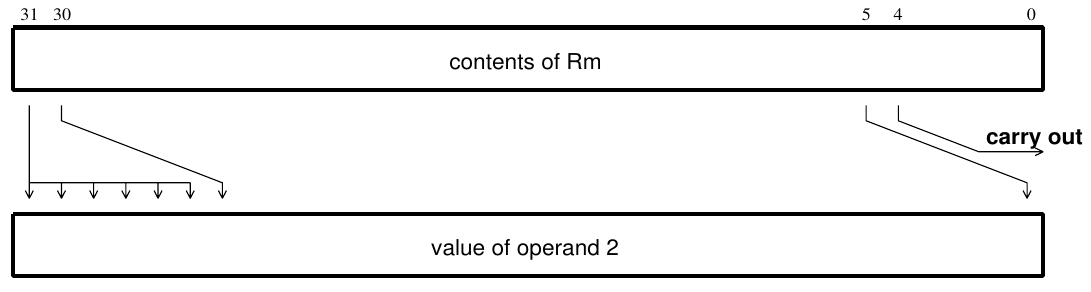
\includegraphics[width=9cm]{pics/asr.png} \\  \hline

\textbf{ROR} & \texttt{ROR N} & Effectue une rotation des bits vers la droite autant de fois que la valeur contenue dans REG. Les bits qui ``débordent'' à droite sont réinsérés à gauche. Le bit qui se retrouverait immédiatement à droite du LSB devient la valeur du drapeau C (\textit{carry}) si le suffixe \textit{S} est utilisé.

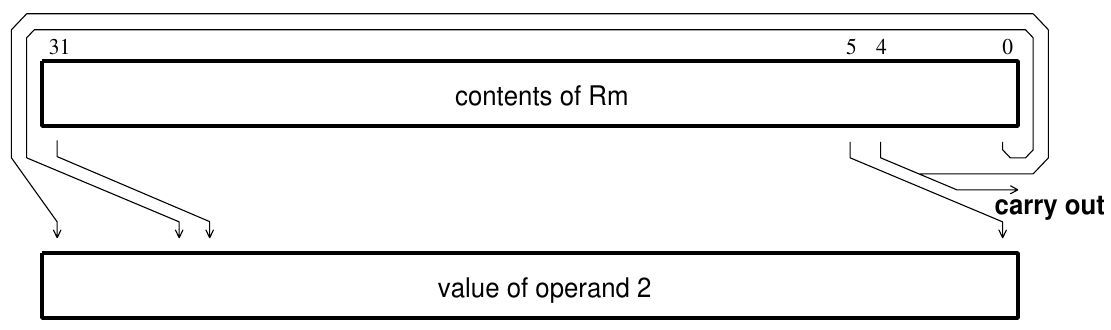
\includegraphics[width=9cm]{pics/ror.png} \\  \hline
  
 \textbf{RRX} & \texttt{RRX} & Opération spéciale qui décale tous les bits du registre vers la droite d'une position. Le drapeau C (\textit{carry}) est inséré à la position du bit le plus significatif (MSB). Le bit éjecté devient la valeur du drapeau C (\textit{carry}) si le suffixe \textit{S} est utilisé. Ce décalage n'accepte pas de paramètre. 
 
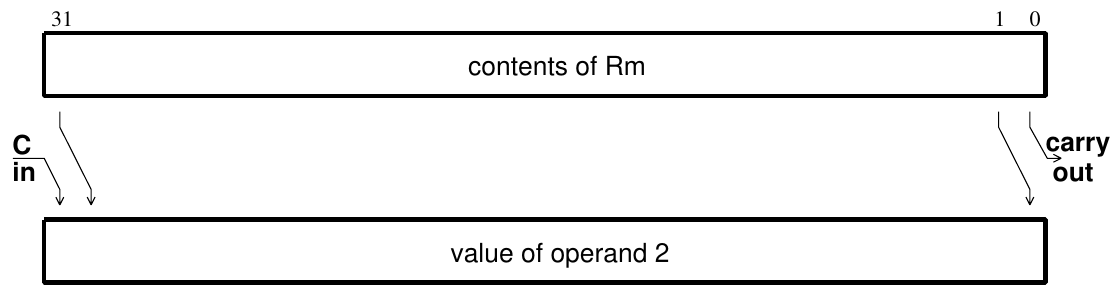
\includegraphics[width=9cm]{pics/rrx.png} \\
\end{tabular}
\label{t:decalage}
\caption{Format des différents modes de décalage acceptés pour une instruction de manipulation de données en ARMv4. $N$ peut être soit un registre, soit une constante positive $\leq 32$. Toutes les figures (sauf RRX) montrent l'effet d'un décalage de $5$.}
\end{table*}



\begin{table*}
\begin{tabular}{l|l|p{7.5cm}l}
Code & Format & Description & Exemple \\ \hline
\textbf{MOV} & \texttt{MOV REG1, REG2[, DEC]} 	& Copie la valeur de REG2 dans REG1. Un décalage optionnel peut être appliqué sur REG2 (voir tableau~\ref{t:decalage}). & \texttt{MOV R1, R2} \\
 			 & \texttt{MOV REG1, \#CONST} 			& Écrit la valeur CONST (en décimal ou hexadécimal précédé de \texttt{0x}) dans REG1 & \texttt{MOV R1, \#0x42} \\
\hline
\textbf{ADD} & \texttt{ADD REG1, REG2, REG3[, DEC]} 	& Additionne REG2 et REG3, stocke le résultat dans REG1. Un décalage optionnel peut être appliqué sur REG3 (voir tableau~\ref{t:decalage}). & \texttt{ADD R1, R2, R3} \\
 			 & \texttt{ADD REG1, REG2, \#CONST} 			& Additionne REG2 et la valeur CONST, stocke le résultat dans REG1 & \texttt{ADD R1, R2, \#42} \\
\hline
\textbf{SUB} & \texttt{SUB REG1, REG2, REG3[, DEC]} 	& Effectue la soustraction REG2 - REG3, stocke le résultat dans REG1. Un décalage optionnel peut être appliqué sur REG3 (voir tableau~\ref{t:decalage}). & \texttt{SUB R1, R2, R3} \\
 			 & \texttt{SUB REG1, REG2, \#CONST} 			& Effectue la soustraction REG2 - CONST, stocke le résultat dans REG1 & \texttt{SUB R1, R2, \#42} \\
\hline
\textbf{RSB} & \texttt{RSB REG1, REG2, REG3[, DEC]} 	& Effectue la soustraction REG3 - REG2, stocke le résultat dans REG1. Un décalage optionnel peut être appliqué sur REG3 (voir tableau~\ref{t:decalage}). & \texttt{RSB R1, R2, R3} \\
 			 & \texttt{RSB REG1, REG2, \#CONST} 			& Effectue la soustraction CONST - REG2, stocke le résultat dans REG1 & \texttt{RSB R1, R2, \#42} \\
\hline

\end{tabular}
\label{t:dataarith}
\caption{Instructions arithmétiques de manipulation de données}
\end{table*}


\begin{table*}
\begin{tabular}{l|l|p{7.5cm}l}
Code & Format & Description & Exemple \\ \hline

\textbf{ADC} & \texttt{ADC REG1, REG2, REG3[, DEC]} 	& Additionne REG2 + REG3 + C, stocke le résultat dans REG1. Un décalage optionnel peut être appliqué sur REG3 (voir tableau~\ref{t:decalage}). & \texttt{ADC R1, R2, R3} \\
 			 & \texttt{ADC REG1, REG2, \#CONST} 			& Additionne REG2 + CONST + C, stocke le résultat dans REG1 & \texttt{ADC R1, R2, \#42} \\
\hline
\textbf{SBC} & \texttt{SBC REG1, REG2, REG3[, DEC]} 	& Effectue la soustraction REG2 - REG3 - 1 + C, stocke le résultat dans REG1. Un décalage optionnel peut être appliqué sur REG3 (voir tableau~\ref{t:decalage}). & \texttt{SBC R1, R2, R3} \\
 			 & \texttt{SBC REG1, REG2, \#CONST} 			& Effectue la soustraction REG2 - CONST - 1 + C, stocke le résultat dans REG1 & \texttt{SBC R1, R2, \#42} \\
\hline
\textbf{RSC} & \texttt{RSC REG1, REG2, REG3[, DEC]} 	& Effectue la soustraction REG3 - REG2 - 1 + C, stocke le résultat dans REG1. Un décalage optionnel peut être appliqué sur REG3 (voir tableau~\ref{t:decalage}). & \texttt{RSC R1, R2, R3} \\
 			 & \texttt{RSC REG1, REG2, \#CONST} 			& Effectue la soustraction CONST - REG2 - 1 + C, stocke le résultat dans REG1 & \texttt{RSC R1, R2, \#42} \\
\hline

\end{tabular}
\label{t:dataarithwithcarry}
\caption{Instructions arithmétiques de manipulation de données utilisant le drapeau Retenue (\textit{Carry}). Dans les explications, $C$ correspond à la valeur de ce drapeau (0 ou 1).}
\end{table*}


\begin{table*}
\begin{tabular}{l|l|p{7.5cm}l}
Code & Format & Description & Exemple \\ \hline
\textbf{MVN} & \texttt{MVN REG1, REG2[, DEC]} 	& Effectue un NON logique sur REG2 et écrit le résultat dans R1. Un décalage optionnel peut être appliqué sur REG2 (voir tableau~\ref{t:decalage}). & \texttt{MVN R1, R2} \\
 			 & \texttt{MVN REG1, \#CONST} 			& Effectue un NON logique sur CONST (inverse ses bits) et écrit le résultat dans REG1 & \texttt{MVN R1, \#42} \\
\hline
\textbf{AND} & \texttt{AND REG1, REG2, REG3[, DEC]} 	& Effectue l'opération ET logique entre REG2 et REG3, stocke le résultat dans REG1. Un décalage optionnel peut être appliqué sur REG3 (voir tableau~\ref{t:decalage}). & \texttt{AND R1, R2, R3} \\
 			 & \texttt{AND REG1, REG2, \#CONST} 			& Effectue l'opération ET logique entre REG2 et CONST, stocke le résultat dans REG1 & \texttt{AND R1, R2, \#0xFF} \\
\hline
\textbf{ORR} & \texttt{ORR REG1, REG2, REG3[, DEC]} 	& Effectue l'opération OU logique entre REG2 et REG3, stocke le résultat dans REG1. Un décalage optionnel peut être appliqué sur REG3 (voir tableau~\ref{t:decalage}). & \texttt{ORR R1, R2, R3} \\
 			 & \texttt{ORR REG1, REG2, \#CONST} 			& Effectue l'opération OU logique entre REG2 et CONST, stocke le résultat dans REG1 & \texttt{ORR R1, R2, \#0xFF} \\
\hline
\textbf{EOR} & \texttt{EOR REG1, REG2, REG3[, DEC]} 	& Effectue l'opération logique REG2 XOR REG3, stocke le résultat dans REG1. Un décalage optionnel peut être appliqué sur REG3 (voir tableau~\ref{t:decalage}). & \texttt{EOR R1, R2, R3} \\
 			 & \texttt{EOR REG1, REG2, \#CONST} 			& Effectue l'opération logique REG2 XOR CONST, stocke le résultat dans REG1 & \texttt{EOR R1, R2, \#0xFF} \\
\hline
\textbf{BIC} & \texttt{BIC REG1, REG2, REG3[, DEC]} 	& Effectue l'opération logique REG2 ET NON REG3, stocke le résultat dans REG1. Un décalage optionnel peut être appliqué sur REG3 (voir tableau~\ref{t:decalage}). & \texttt{BIC R1, R2, R3} \\
 			 & \texttt{BIC REG1, REG2, \#CONST} 			& Effectue l'opération logique REG2 et NON CONST, stocke le résultat dans REG1 & \texttt{BIC R1, R2, \#0xFF} \\
\hline

\end{tabular}
\label{t:databool}
\caption{Instructions booléennes de manipulation de données}
\end{table*}



\begin{table*}
\begin{tabular}{l|l|p{7.5cm}l}
Code & Format & Description & Exemple \\ \hline
 \textbf{CMP} & \texttt{CMP REG1, REG2[, DEC]} 	& Effectue la soustraction REG1 - REG2 et met à jour les drapeaux en fonction du résultat. Un décalage optionnel peut être appliqué sur REG2 (voir tableau~\ref{t:decalage}). & \texttt{CMP R1, R2} \\
 			 & \texttt{CMP REG1, \#CONST} 			& Effectue la soustraction REG1 - CONST et met à jour les drapeaux en fonction du résultat. & \texttt{CMP R1, \#18} \\ \hline
\textbf{CMN} & \texttt{CMN REG1, REG2[, DEC]} 	& Effectue l'addition REG1 + REG2 et met à jour les drapeaux. Un décalage optionnel peut être appliqué sur REG2 (voir tableau~\ref{t:decalage}). & \texttt{CMN R1, R2} \\
 			 & \texttt{CMN REG1, \#CONST} 			& Effectue l'addition REG1 + CONST et met à jour les drapeaux en fonction du résultat. & \texttt{CMN R1, \#18} \\
\hline
\textbf{TEQ} & \texttt{TEQ REG1, REG2[, DEC]} 	& Effectue l'opération logique REG1 XOR REG2 et met à jour les drapeaux en fonction du résultat. Un décalage optionnel peut être appliqué sur REG2 (voir tableau~\ref{t:decalage}). & \texttt{TEQ R1, R2} \\
 			 & \texttt{TEQ REG1, \#CONST} 			& Effectue l'opération logique REG1 XOR CONST et met à jour les drapeaux en fonction du résultat. & \texttt{TEQ R1, \#0x5F} \\
\hline
\textbf{TST} & \texttt{TST REG1, REG2[, DEC]} 	& Effectue l'opération logique REG1 AND REG2 et met à jour les drapeaux en fonction du résultat. Un décalage optionnel peut être appliqué sur REG2 (voir tableau~\ref{t:decalage}). & \texttt{TST R1, R2} \\
 			 & \texttt{TST REG1, \#CONST} 			& Effectue l'opération logique REG1 AND CONST et met à jour les drapeaux en fonction du résultat. & \texttt{TST R1, \#0x5F} \\ \hline

\end{tabular}
\label{t:datacmp}

\caption{Instructions de comparaisons de données (arithmétique et logique). Ces instructions ont le même effet que d'autres, mais n'écrivent leur résultat nulle part -- elles ne font qu'agir sur les drapeaux. Pour cette raison, le suffixe \textit{S} est redondant et ne doit pas être utilisé.}
\end{table*}

\clearpage
\section{Assignations et allocations en mémoire}

Écrire une instruction réserve implicitement 4 octets en mémoire. Toutefois, il est également possible de réserver ou assigner des valeurs arbitraires à n'importe quel endroit dans la mémoire. Deux mots clés sont disponibles à cette fin. Il est à noter que ces mots clés \textbf{ne sont pas des instructions} : ils ne génèrent aucun code ARM en tant que tel, mais se contentent d'initialiser ou de réserver certaines sections de la mémoire. Ces directives doivent être précédées d'une étiquette qui sert de nom de variable.

\begin{itemize}
	\item Le mot clé \texttt{ALLOC} permet \textbf{d'allouer} une certaine quantité de mémoire, sans l'initialiser (c'est-à-dire que vous ne pouvez pas déterminer ses valeurs initiales). Sa syntaxe est \texttt{ALLOCT NOMBRE}, où \texttt{T} est un nombre déterminant la taille des éléments à allouer et \texttt{NOMBRE} le nombre d'éléments de cette taille à allouer. \texttt{T} est exprimé en bits, et peut prendre les valeurs 8, 16 ou 32. 
	
	Par exemple, la ligne \texttt{mavariable ALLOC32 5} allouera 5 espaces de 32 bits (4 octets) chacun; l'étiquette \textit{mavariable} permettra d'y faire référence dans le code. De même \texttt{monoctet ALLOC8 1} allouera 1 espace de 8 bits, soit un octet au total, avec \textit{monoctet} comme étiquette de référence.
	
	\item Le mot clé \texttt{ASSIGN} permet \textbf{d'assigner} une valeur à une ou plusieurs adresses mémoire. Sa syntaxe est \texttt{ASSIGNT VAL1, VAL2, ..., VALN}, où \texttt{T} est un nombre déterminant la taille des éléments en mémoire et \texttt{VAL1, VAL2, ..., VALN} une liste de valeurs séparées par des virgules de longueur arbitraire, qui seront écrites à la suite dans la mémoire. Tout comme pour \texttt{ALLOC}, \texttt{T} est exprimé en bits, et peut prendre les valeurs 8, 16 ou 32. 
	
	Par exemple, la ligne \texttt{mavariable ASSIGN32 8, 0x12, 0, -1} assignera la valeur 8 (représentée sur 32 bits) aux 4 premiers octets, la valeur 0x12 aux 4 suivants, la valeur 0 aux 4 suivants et la valeur -1 aux 4 suivants, pour un total de 16 octets assignés.
	
	La directive \texttt{ASSIGN} accepte également des chaînes de caractères écrites entre guillemets. Par exemple, la ligne \texttt{machaine ASSIGN8 "ceci est du texte"} assignera un octet pour chaque caractère ASCII du texte contenu entre les guillements.
\end{itemize}

Notons qu'une étiquette ne peut être déclarée ou assignée \textbf{qu'une seule fois}. Par exemple, faire suivre \texttt{mavariable ALLOC32 5} de \texttt{mavariable ASSIGN32 8, 0x12, 0, -1} est une erreur, puisque \texttt{mavariable} est alors utilisée deux fois.

\clearpage
\section{Instructions d'accès mémoire}
\vspace{-0.8em}
\subsection{Accès mémoire de base}

Il existe deux types d'accès mémoire (avec leur mnémonique) :
\begin{itemize}
	\item \texttt{LDR}, qui lit une donnée de la mémoire et l'écrit dans un registre;
	\item \texttt{STR}, qui lit un registre et écrit sa valeur dans la mémoire;
\end{itemize}

Plusieurs suffixes peuvent être ajoutés à ces opérations pour modifier leur comportement (en plus du suffixe conditionnel) :
\begin{itemize}
	\item Le suffixe \texttt{B}, qui permet de ne lire qu'un seul octet (au lieu de 4)
	\item Le suffixe \texttt{H}, qui permet de ne lire que 2 octets (au lieu de 4)
	\item Dans le cas de LDR, les suffixes \texttt{SB} et \texttt{SH}, qui lisent respectivement 1 et 2 octets, mais en \textit{étendant le signe de la valeur lues au reste du registre}. Par exemple, lire la valeur $0xFF$ en mode \texttt{B} écrira la valeur $0x000000FF$ dans le registre de destination. Faire la même chose en mode \texttt{SB} écrira plutôt $0xFFFFFFFF$ (le MSB de l'octet lu est dupliqué à gauche).
\end{itemize}
Note : l'utilisation des suffixes \texttt{H}, \texttt{SH} ou \texttt{SB} empêche l'utilisation des cas 3, 5, 6 et 7 de la liste suivante ou d'un décalage.

\subsection{Format d'une instruction LDR ou STR}

Les instructions d'accès mémoire sont du format : \texttt{LDR REG, INFOMEM} où REG est le registre source (dans le cas de STR) ou de destination (dans le cas de LDR), et INFOMEM une expression déterminant une adresse mémoire. Celle-ci peut prendre sept formes :
\begin{enumerate}
	\item {[REGBASE] : la valeur contenue dans REGBASE est directement interprétée comme une adresse}
	\item {[REGBASE, REGADD] : les valeurs de REGBASE et REGADD sont additionnées pour former une adresse. REGADD peut optionnellement être décalé, mais seulement par constante (voir tableau \ref{t:decalage}). Si le ] est suivi d'un point d'exclamation (!), la somme de REGBASE et REGADD est écrite dans REGBASE par après}
	\item {[REGBASE, \#CONST] : les valeurs de REGBASE et CONST sont additionnées pour former une adresse. Un point d'exclamation peut ici aussi être ajouté pour stocker la somme dans REGBASE}
	\item {[REGBASE], REGADD : la valeur de REGBASE est utilisée comme adresse, mais REGADD est additionné à cette valeur \textit{après} l'accès mémoire, et le résultat stocké dans REGBASE. REGADD peut optionnellement être décalé (voir tableau \ref{t:decalage}), mais seulement par constante (pas par registre)}
	\item {[REGBASE], \#CONST : la valeur de REGBASE est utilisée comme adresse, mais CONST est additionné à cette valeur \textit{après} l'accès mémoire, et le résultat stocké dans REGBASE}
	\item LABEL : l'assembleur transforme l'étiquette LABEL en un accès relatif à PC. L'étiquette doit être définie ailleurs dans le programme.
	\item =LABEL : l'assembleur transforme =LABEL en un accès relatif à PC vers \textit{l'adresse} de l'étiquette LABEL (l'équivalent d'un pointeur en C). Cette étiquette doit être définie ailleurs dans le programme. Ce mode ne peut être utilisé qu'en conjonction avec \texttt{LDR} (il est interdit de l'utiliser avec une instruction \texttt{STR}).
\end{enumerate}

\subsection{Exemples d'utilisation}

\paragraph{\texttt{LDR R0, [R1]}} Copie dans R0 la valeur contenue dans l'adresse mémoire désignée par R1 et les 3 octets suivants (4 octets au total).

\paragraph{\texttt{LDR R0, [R1, \#4]}} Copie dans R0 la valeur contenue dans l'adresse mémoire calculée par R1+4 et les 3 octets suivants (4 octets au total).

\paragraph{\texttt{LDR R0, [R1, R2]}} Copie dans R0 la valeur contenue dans l'adresse mémoire calculée par R1+R2 et les 3 octets suivants (4 octets au total).

%\paragraph{\texttt{LDR R0, [R1, R2, LSL R3]}} Copie dans R0 la valeur contenue dans l'adresse mémoire calculée par R1+N et les 3 octets suivants (4 octets au total), où N est la valeur de R2 décalée vers la gauche R3 fois.

\paragraph{\texttt{LDR R0, [R1, R2, LSR \#2]}} Copie dans R0 la valeur contenue dans l'adresse mémoire calculée par R1+N et les 3 octets suivants (4 octets au total), où N est la valeur de R2 décalée deux fois vers la droite.

\paragraph{\texttt{LDR R0, [R1, R2]!}} Copie dans R0 la valeur contenue dans l'adresse mémoire calculée par R1+R2 et les 3 octets suivants (4 octets au total). Par la suite, stocke le résultat de R1+R2 dans R1.

\paragraph{\texttt{LDRB R0, [R1]}} Copie dans R0 la valeur de l'octet contenu dans l'adresse mémoire désignée par R1.

\paragraph{\texttt{LDRGEB R0, [R1], R2}} Copie dans R0 la valeur de l'octet contenu dans l'adresse mémoire désignée par R1. Additionne R1+R2 et stocke le résultat dans R1. Ces opérations ne sont effectuées que si la condition GE est rencontrée.

\paragraph{\texttt{LDR R0, mavariable}} Copie dans R0 la valeur contenue dans l'adresse mémoire désignée par l'étiquette \textit{mavariable} et les 3 octets suivant.

\paragraph{\texttt{LDR R0, =var2}} Copie dans R0 \textit{l'adresse de} l'étiquette \textit{var2}.

\paragraph{\texttt{LDRH R0, [R1]}} Copie dans R0 la valeur contenue dans l'adresse mémoire désignée par R1 et l'octet suivant (2 octets au total).

\paragraph{\texttt{STR R0, [R1]}} Copie les 4 octets composant la valeur de R0 à l'adresse mémoire désignée par R1 (ainsi que les 3 octets suivants).

\paragraph{\texttt{STRB R0, [R1]}} Copie l'octet le moins significatif de la valeur de R0 à l'adresse mémoire désignée par R1.

\paragraph{\texttt{STREQ R0, [R1], \#8}} Copie l'octet le moins significatif de la valeur de R0 à l'adresse mémoire désignée par R1. Additionne 8 à R1 et stocke le résultat dans R1. Ces opérations ne sont effectuées que si la condition EQ est rencontrée.

\paragraph{\texttt{STR R0, mavariable}} Copie les 4 octets composant la valeur de R0 à l'adresse mémoire désignée par l'étiquette \textit{mavariable}.


\subsection{Accès mémoire multiples}

Il est également possible de lire ou écrire plusieurs espaces mémoire contigus simultanément. De manière générale, ce genre d'accès est surtout utilisé en conjonction avec une pile. Les instructions à utiliser sont \texttt{PUSH} et \texttt{POP}. Ces deux instructions prennent une liste de registre en paramètre, entourés d'accolages (\{\}). Les registre listés sont stockés dans la mémoire, de la manière suivante :
\begin{enumerate}
	\item Le registre SP (R13) est décrémenté de 4 octets
	\item La valeur du registre dont l'index est \textbf{le plus élevé} est stockée à cette adresse (par exemple, si on a R5, R8 et R11, c'est la valeur de R11 qui sera écrite).
	\item Le registre SP est décrémenté de quatre octets, et le cycle recommence avec les registres restant à écrire.
\end{enumerate}
L'utilisation de POP est similaire, mais la mémoire est lue au lieu d'être écrite et SP incrémenté au lieu d'être décrémenté. L'ordre des registres dans la liste n'a donc aucune importance, seule leur présence (ou absence) est prise en compte.

\subsection{Exemples d'utilisation}

\paragraph{\texttt{PUSH \{R0, R3-R7\}}} Stocke les registres R0, R3, R4, R5, R6 et R7 à partir de l'adresse pointée par SP (en descendant la mémoire)

\paragraph{\texttt{POPNE \{R4, R5, R12\}}} Lit la mémoire et copie ses valeurs dans R4, R5 et R12 à partir de l'adresse pointée par SP (en remontant la mémoire), mais seulement si la condition NE est rencontrée.

\subsection{Échange mémoire/registre (swap)}

Un dernier type d'accès, plus rare, est un accès \textit{d'échange}, qui écrit et lit simultanément le même espace mémoire. L'instruction à utiliser est \textit{SWP}, dont la syntaxe est la suivante : \texttt{SWP REG1, REG2, [REG3]}. REG3 doit contenir l'adresse où l'on souhaite lire et écrire, REG2 le contenu que l'on souhaite y écrire et REG1 le registre de destination pour la valeur lue. La valeur est lue dans REG1 avant d'être modifiée par l'écriture de REG2. Un suffixe \texttt{B} peut optionnellement être ajouté pour ne lire/écrire qu'un seul octet (au lieu de 4).

\subsection{Exemples d'utilisation}

\paragraph{\texttt{SWP R3, R8, [R9]}} Copie la valeur contenue à l'adresse mémoire contenue dans R9 dans R3, écrit la valeur de R8 à cette même adresse

\paragraph{\texttt{SWPPLB R1, R2, [R10]}} Copie la valeur de l'octet contenu à l'adresse mémoire contenue dans R10 dans R1, écrit la valeur de l'octet le moins significatif de R8 à cette même adresse, mais seulement si la condition PL est rencontrée

\clearpage
\section{Instructions de branchement}

Ces instructions permettent de modifier la valeur de PC afin de changer le fil d'exécution du programme. Elles sont souvent utilisées en conjonction avec une condition pour réaliser un bloc \textit{IF}. Il existe trois types d'instruction de branchement :
\begin{enumerate}
	\item \texttt{B LABEL}, qui assigne PC à l'adresse de l'étiquette LABEL
	\item \texttt{BL LABEL}, qui opère la même opération, mais stocke de plus l'adresse de l'instruction \textit{suivant le BL} dans le registre LR (R14). Cette instruction est souvent utilisée pour appeler une fonction en conservant l'adresse de retour.
	\item \texttt{BX REG}, qui copie la valeur du registre REG dans PC. Cette instruction est souvent utilisée avec le registre LR pour revenir d'une fonction.
\end{enumerate}

\subsection{Exemples d'utilisation}

\paragraph{\texttt{B main}} Branche inconditionnellement à l'adresse de l'étiquette \textit{main}

\paragraph{\texttt{BEQ maboucle}} Branche à l'adresse de l'étiquette \textit{maboucle}, mais seulement si la condition EQ est remplie

\paragraph{\texttt{BL mafonction}} Branche inconditionnellement à l'adresse de l'étiquette \textit{mafonction}, écrit l'adresse de l'instruction suivant ce \texttt{BL} dans le registre LR

\paragraph{\texttt{BX LR}} Copie la valeur de LR dans PC et poursuit l'exécution

\paragraph{\texttt{BXLE R3}} Copie la valeur de R3 dans PC, mais seulement si la condition LE est rencontrée

\clearpage
\section{Instructions de décalage}

On peut utiliser une instruction \texttt{MOV} pour réaliser n'importe quel type de décalage. Toutefois, pour faciliter la programmation, un ensemble de cinq \textit{pseudo-instructions} sont fournies et permettent d'écrire directement une opération de décalage :

\begin{itemize}
	\item \texttt{LSL REG1, REG2, REG3} ou \texttt{LSL REG1, REG2, \#CONST} : décale REG2 de REG3 ou \#CONST positions vers la gauche, stocke le résultat dans REG1. Équivalent à \texttt{MOV REG1, REG2, LSL REG3}.
	\item \texttt{LSR REG1, REG2, REG3} ou \texttt{LSR REG1, REG2, \#CONST} : décale REG2 de REG3 ou \#CONST positions vers la droite, stocke le résultat dans REG1. Équivalent à \texttt{MOV REG1, REG2, LSR REG3}.
	\item \texttt{ASR REG1, REG2, REG3} ou \texttt{ASR REG1, REG2, \#CONST} : décale REG2 de REG3 ou \#CONST positions vers la droite (en copiant la valeur du MSB sur tous les bits insérés), stocke le résultat dans REG1. Équivalent à \texttt{MOV REG1, REG2, ASR REG3}.
	\item \texttt{ROR REG1, REG2, REG3} ou \texttt{ROR REG1, REG2, \#CONST} : décale REG2 de REG3 ou \#CONST positions vers la droite en réinsérant les bits à la gauche du registre, stocke le résultat dans REG1. Équivalent à \texttt{MOV REG1, REG2, ROR REG3}.
	\item \texttt{RRX REG1, REG2} : décale REG2 de une position vers la droite en utilisant le drapeau Retenue (C) comme nouvelle valeur de MSB. Équivalent à \texttt{MOV REG1, REG2, RRX}.
\end{itemize}

Note : ces instructions étant des pseudo-instructions, leur encodage est strictement le même qu'une instruction MOV équivalente. Le tableau \ref{t:decalage} présente en détails chaque type de décalage.

\subsection{Exemples d'utilisation}

\paragraph{\texttt{LSL R9, R10, R4}} Décale R10 de R4 positions vers la gauche, stocke le résultat dans R9

\paragraph{\texttt{LSREQ R1, R2, \#6}} Décale R2 de 6 positions vers la droite, stocke le résultat dans R1, mais seulement si la condition EQ est rencontrée.



\clearpage
\section{Instructions d'accès au registre de contrôle et de statut}

Deux instructions permettent d'accéder et de modifier les registres de contrôle et de statut (CPSR et SPSR). Ces instructions sont les suivantes :

\begin{itemize}
	\item \texttt{MRS REG, STATUS} : transfère la valeur du registre STATUS (qui peut être CPSR ou SPSR) dans le registre REG
	\item \texttt{MSR STATUS, REG} : transfère la valeur du registre REG dans le registre STATUS (qui peut être CPSR ou SPSR)
	\item \texttt{MSR STATUS\_flg, REG} ou \texttt{MSR STATUS\_flg, \#CONST} : transfère la valeur du registre REG ou de la constante CONST dans le registre STATUS (qui peut être CPSR ou SPSR), mais ne fait que agir sur les drapeaux (les autres bits du registre de statut ne sont pas modifiés)
\end{itemize}

Attention : l'accès au registre SPSR n'est valide que dans les modes qui en comportent un.

\subsection{Exemples d'utilisation}

\paragraph{\texttt{MRS R9, CPSR}} Transfère le contenu du registre CPSR dans le registre R9

\paragraph{\texttt{MRS SPSR, R5}} Transfère le contenu du registre R5 dans le registre SPSR du mode courant


\paragraph{\texttt{MRS CPSR\_flg, \#0xF0000000}} Transfère la constante 0xF0000000 dans le registre CPSR, mais en n'affectant que les drapeaux. Les drapeaux étant aux bits 28 à 31 du CPSR, cette instruction les assigne tous à 1.

\clearpage
\section{Instructions de déclenchement d'une interruption logicielle}

Deux mnémoniques équivalentes permettent de déclencher une interruption logicielle : \texttt{SWI} et \texttt{SVC}. Ces instructions possèdent \textit{exactement} le même comportement et prennent en paramètre une constante dont la valeur ne peut excéder $2^24$. Cette valeur est ignorée par le processeur, mais peut être récupérée par l'interruption logicielle et être utilisée comme paramètre.

\subsection{Exemples d'utilisation}

\paragraph{\texttt{SVC \#0xCAFE}} Déclenche une interruption logicielle
\paragraph{\texttt{SWI \#22}} Déclenche une interruption logicielle
\paragraph{\texttt{SVCEQ \#0xCAFE}} Déclenche une interruption logicielle seulement si la condition EQ est rencontrée


\clearpage
\section{Assertions}

En plus des instructions ARM et des directives de déclarations mémoire, le simulateur supporte un mécanisme \textit{d'assertion} qui permet de valider le fonctionnement d'un programme. Il se base sur une directive spéciale, \texttt{ASSERT}. Lorsque le simulateur rencontre une ligne contenant ce mot-clé, il évalue la ou les expressions qui suivent. Si ces expressions ne sont pas vraies, il arrête la simulation et écrit un message d'erreur indiquant les divergences entre le résultat prévu et obtenu. Si les expressions sont vraies, aucune action n'est prise et le programme se poursuit normalement. On peut combiner plusieurs expressions sur la même ligne en les séparant par des virgules et ces expressions peuvent être de trois types :
\begin{itemize}
	\item Vérification d'un registre : \texttt{REG=VAL}, où \texttt{REG} est un registre et \texttt{VAL} la valeur qu'il doit posséder, en décimal ou hexadécimal.
	\item Vérification d'une adresse mémoire : \texttt{ADDR=VAL}, où \texttt{ADDR} est une adresse mémoire commençant par \texttt{0x} et \texttt{VAL} la valeur que cette case mémoire doit posséder. Si \texttt{VAL} est entre 0 et 255, seule l'octet pointé par cette adresse est comparé; sinon, ce sont aussi les trois octets suivants qui sont comparés (pour une taille totale de 32 bits ou 4 octets)
	\item Vérification d'un drapeau : \texttt{DRAPEAU=VAL}, où \texttt{DRAPEAU} est une lettre \textit{majuscule} désignant un drapeau (C, V, Z ou N) et \texttt{VAL} la valeur (0 ou 1) attendue
\end{itemize}

\subsection{Exemples d'utilisation}

\paragraph{\texttt{ASSERT R0=9}} Teste si R0 vaut bel et bien 9

\paragraph{\texttt{ASSERT R2=0x18, R1=-5}} Teste si R2 vaut bel et bien 0x18 et R1 -5

\paragraph{\texttt{ASSERT 0x16=24}} Teste si la valeur à l'adresse 0x16 de la mémoire est bien 24

\paragraph{\texttt{ASSERT 0x1004=-1}} Teste si les valeurs aux adresses 0x1004 à 0x1007 inclusivement valent bien -1 (0xFFFFFFFF)

\paragraph{\texttt{ASSERT C=1,Z=0}} Teste si le drapeau Retenue (\textit{Carry}) est bien levé et le drapeau Zéro inactif


\subsection{Note importante}

Les assertions ne sont pas des instructions ARM et n'apparaissent donc pas dans le bytecode. Elles ne peuvent pas être copiées d'un endroit à l'autre de la mémoire comme le peuvent être des instructions.

\clearpage
\section{Remerciements}

Les auteurs tiennent à remercier les personnes suivantes pour l'aide qu'ils ont apporté à la réalisation de ce simulateur :
\begin{itemize}
	\item Jessica Déziel, pour le design de l'interface graphique
	\item Jonathan Gilbert, pour les tests préliminaires du simulateur et la réalisation des exercices
	\item Étienne Dubeau, pour son travail à l'amélioration du simulateur et à l'implémentation de nouvelles fonctionnalités
\end{itemize}

\end{document} 
